\chapter{Pilottest}
\label{TestAfSkalaPilottest}
%
Da der er foretaget ændringer i testdesignet i forhold til det testdesign der blev brugt i feltundersøgelsen vil der udføres nogle pilottests. Alle pilottest er udført på Aalborg Universitet Fredrik Bajers vej 7B i projektgruppens grupperum. Til hver pilottest er der både en robotstyrer, en observatør som holder øje med hvad testpersonerne trykker på, en testleder, som præsenterer skalaerne samt en observatør, der sørger for at notere pilottestens forløb.  

\subsubsection*{Pilottest 1}
\label{TestAfSkalaerPilot1}
%
Den første pilottest blev udført af en mand på 25 år, som læser Produkt- og Designpsykologi. Da programmet til præsentation af skalaer endnu ikke var færdigudviklet blev skalaerne præsenteret i udprintet form på A4 papir. Skalaerne blev præsenteret efter samme rækkefølge som hvis de blev præsenteret på computeren.

Robotten henvendte sig til testpersonen ude på gangen foran grupperummet og kørte tæt på testpersonen, som kommenterede at robotten kom lidt for tæt på, hvorfor testpersonen rykkede et skridt tilbage. Robottens højde var indstillet til albuehøjde, svarende til 129 cm. 

Testlederen introducerede skalaerne med et meget formelt ordvalg, som for testpersoner, der ikke har samme faglige baggrund som projektgruppen, kan have svært ved at forstå. Derudover undskyldte testlederen flere gange ved at sige: \textit{Jeg er ked af at sige det}, hvilket giver en lidt mærkelige stemning. Der skal ikke undskyldes for hvorfor testen er bygget op som den er, det virker useriøst og som om at der er problemer med hvordan testen afvikles. Derudover blev det bemærket at testlederen havde en tendens til at stå bag testpersonen, når testpersonen svarede på skalaerne, hvilket ikke hensigtsmæssigt, da det kan virke som om at testlederen overvåger testpersonens besvarelser.\blankline
%
Testpersonen var i tvivl om hvordan skala spørgsmålet: \textit{Hvordan synes du, at skærmen på robotten reagerede?} skulle forståes. Testpersonen var i tvivl om hvorvidt spørgsmålet handlede om hvordan det var at trykke på skærmen eller om det handlede om hvorvidt valgmulighederne var tilfredstillende. Årsagen til at tvivlen kan være opstået er formentlig, at testpersonen ikke oplevede problemer med at interagere på robottens skærm. Det vælges ikke, at omformulere spørgsmålet da det forventes, at en del danske rejsende vil opleve problemer med skærmen når testen afvikles i Aalborg Lufthavn. 

En anden ting testpersonen var i tvivl om var hvad ordet \textit{anmassende} betød. Testlederen fortæller, at det er testpersonens forståelse af ordet \textit{anmassende}, der skal evalueres ud fra, hvorefter testpersonen begynder, at forklare ordets betydning. Baseret på den forklaring er det klart, at testpersonen har forstået hvad der menes med \textit{anmassende}, nemlig at robotten kommer meget tæt på, og presse på ved at køre lidt ind i testpersonen. Dog forklarer testpersonen, at hvis robotten blev ved med at være tæt på ville det føles \textit{anmassende}, men da robotten efterfølgende holdte afstand føltes det ikke \textit{anmassende}.

Derudover kommenterer testpersonen på ordet \textit{sjov} i forhold til det er meget subjektivt hvad der forståes ved ordet \textit{sjovt}. Testpersonen selv synes ikke, at robotten var \textit{sjov sjov}, hvor det virker som om den formulering afspejler noget, der får en til at grine.

\subsubsection*{Pilottest 2}
\label{TestAfSkalaerPilot2}
%
Den anden pilottest blev udført at gruppens kvindelige vejleder. Da programmet endnu ikke er færdigudviklet og der ikke var tid til at printe et nyt sæt skalaer, foreslog vejlederen, at de udprintede skalaer fra den forrige pilottest bare kunne bruges igen. 

Testpersonen har mange problemer med skærmen i begyndelsen af interaktionen, hvor den ikke reagerer på tryk. Det bør derfor overvejes om der bør tilføjes noget tekst på skærmen, hvorpå der står, at der skal trykkes på en bestemt måde. Igen undskylder testlederen flere gange overfor testpersonen, hvilket ikke er hensigtsmæssigt og testlederen bruger stadig et meget formelt sprog. Et forslag til hvordan testlederen starter samtalen med testpersonen er, at testlederen siger noget i stil med: \textit{Du har lige snakket med den her robot, og jeg vil gerne vide lidt om din oplevelse}, på den måde undgåes det formelle ordvalg. 

Derudover bliver testpersonen fortalt, at der er 24 skalaer de skal svare på. Dette bør undgåes da 24 lyder af mange og det kan være svært at forholde sig til og så er det heller ikke meningen at testpersonen skal holde styr på hvor mange skalaer, der er besvaret og hvor mange der er igen.\blankline     
%
Testpersonen er i tvivl om hvad der menes med ordet: \textit{personlig} i forhold til skala spørgsmålet: \textit{Hvor personlig oplevede du robottens hjælp?}, om det er i forhold til testpersonen selv. Testlederen forklarer, at det er hvad testpersonen forstår ved ordet, der skal svares ud fra.

De otte skalaer, som hører til skala spørgsmålet: \textit{Hvad synes du om robotten?}, er ligeligt fordelt på to papirer, ligesom det på computeren vil være fordelt på to skærmbilleder, hvorfor skala spørgsmålet vil være på begge sider. Dette kommenterede testpersonen var forvirrende, da det kunne opleves som om, at der var opstået en fejl, så skalaerne skulle besvares igen. Testpersonen foreslår at lave en anden overskrift til de fire sidste skalaer, hvor overskrift henviser til skala spørgsmål.

Derudover kommenterer testpersonen at det er abstrakt og svært at forholde sig til spørgsmålet: \textit{Hvad er din kendskab til teknologi?}, hvorfor dette bør revurderes. Efter en dialog med projektgruppen bliver det foreslået, at ændre spørgsmålet til: \textit{Hvor glad er du for teknologi?}, da det egentlig er det, projektgruppen gerne vil vide. Der bliver også diskuteret om der skal spørges ind til om testpersonerne har let ved at bruge sin smartphone eller sin computer, og i det henseende hvornår de sidst købte en ny. 

\subsubsection*{Pilottest 3}
\label{TestAfSkalaerPilot3}
%
Tredje pilottest blev udført af en mand på 25 år, som læser Produkt- og Designpsykologi, hvor skalaerne besvares på computeren, igennem det udviklede program. 

Igen nævner testlederen hvor mange skalaer, der er og i tillæg hvor langtid det kommer til at tage. Problemet med at nævne tiden i pilottesten er, at det er første gang programmet bliver brugt, så det vides ikke hvor lang tid det kan komme til at tage, og derudover afhænger det af, hvor hurtig testpersonen er til at besvare skalaerne. Testlederen står bag testpersonen hvilket for testpersonen kan virke overvågende, årsagen er dog, at programmet ikke er testet før og for at sikre, at programmet fungerer står testlederen bag ved. Derudover oplever testpersonen problemer med at respondere på skalaerne på computeren.   

\section{Ændringer efter pilottest}
\label{TestAfSkalaerAendringerPilot}
%
Baseret på de tre pilottests vil der foretages ændringer til testen. Testlederen skal sørger for ikke, at bruge formelt sprog, ikke nævne antallet af skalaer eller undskylde, at testen er som den er. Så vidtmuligt skal testlederen følge instruktionerne beskrevet i \fullref{TestAfSkalaFremgangsmaade}.

Da der både i feltundersøgelsen og i de før beskrevne pilottest gentagende gange er oplevet problemer med robottens skærm, vælges det er at tilføje en tekst på det første skærmbillede, hvor der står: \textit{Tryk blidt på mig}, da det er fundet, at hvis der trykkes meget blidt på skærmen så reagerer den. På \autoref{fig:ForsideRettet} fremgår ændringen på det første skærmbillede, hvor teksten er tilføjet.    
%
\begin{figure}[H]
\centering

\includegraphics[width = 0.3\textwidth]{Figure/TestdesignEvaluering/ForsideRettet} 
\caption{Ændringen til den første side, der præsenteres på robotten, hvor der tilføjet den grå tekst: \textit{Tryk blidt på mig}.}
\label{fig:ForsideRettet}
\end{figure}
\noindent
%
Baseret på pilottest 2, hvor det blev besluttet at ændre spørgmålet: \textit{Hvad er din kendskab til teknologi?} til: \textit{Hvor glad er du for teknologi?}, i demografien. I det henseende vælges det at præsentere spørgsmålet som et skala spørgsmål, hvor testpersonerne angiver hvor glade de er for teknologi på en unipolær VAS med lukkede endepunkter fra: \textit{Slet ikke glad} til: \textit{Ekstremt glad}. Før ændringen skulle testpersonerne både angive hvor ofte de gennemsnitligt rejse og hvad deres kendskab til teknologi er på en Likert-skala med fem valgmuligheder. Da spørgsmålet omkring teknologi er ændret til et skala spørgsmål med tilhørende skala, vælges det ligeledes at ændre både formuleringen og måden hvorpå \textit{Hvor ofte rejser du i gennemsnit?} præsenteres. Spørgsmålet omformuleres til: \textit{Angiv hvor mange gange du ca. flyver på et år}, hvilket skal besvares på samme måde som alder og højde. Ændringerne til demografi fremgår på \autoref{fig:TilpassetDemografi}.
%
\begin{figure}[H]
\centering
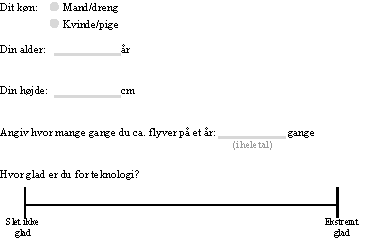
\includegraphics[width = 0.7\textwidth]{Figure/TestdesignEvaluering/TilpassetDemografi} 
\caption{Ændringer til demografi.}
\label{fig:TilpassetDemografi}
\end{figure}
\noindent
%
Den sidste ændring, der er foretaget på baggrund af pilottestene er, at ændre skala spørgsmålet: \textit{Hvad synes du om robotten?}, på side to, så der ikke opstår forvirring. Skala spørgsmålet på side to vil fremover være: \textit{Hvad synes du eller om robotten?}. Første side fremgår på \autoref{fig:TilpassetHvadSynesDuOmR}, hvor anden side fremgår på \autoref{fig:TilpassetHvadSynesDuEllersOmR}.  
%
\begin{figure}[H]
\centering
\begin{minipage}{.5\textwidth}
  \centering
  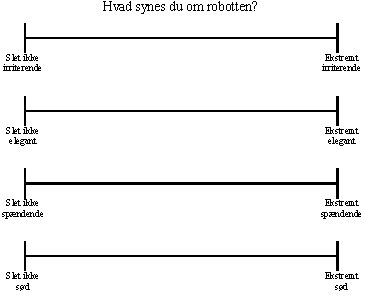
\includegraphics[width=\linewidth]{Figure/TestdesignEvaluering/TilpassetHvadSynesDuOmR}
  \caption{Første side med de otte skalaer.}
  \label{fig:TilpassetHvadSynesDuOmR}
\end{minipage}%
\begin{minipage}{.5\textwidth}
  \centering
  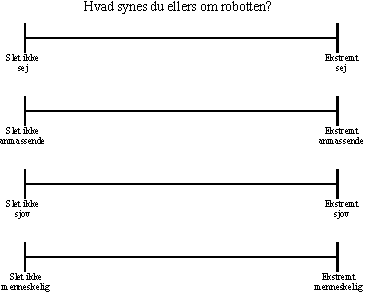
\includegraphics[width=\linewidth]{Figure/TestdesignEvaluering/HvadSynesDuEllersOmR}
  \caption{Anden side med de otte skalaer.}
  \label{fig:TilpassetHvadSynesDuEllersOmR}
\end{minipage}
\end{figure}
\noindent
%
